\documentclass[a4paper,10pt]{article}
\usepackage[margin=0.6cm]{geometry}
\usepackage{tikz}
\usetikzlibrary{arrows,shapes,positioning,shadows,trees,fit}

\begin{document}
\pagestyle{empty}

\begin{center}
\textbf{\Large ROS2 Robotics Control Architecture}
\end{center}

\begin{figure}[h]
\centering
\resizebox{\textwidth}{!}{%
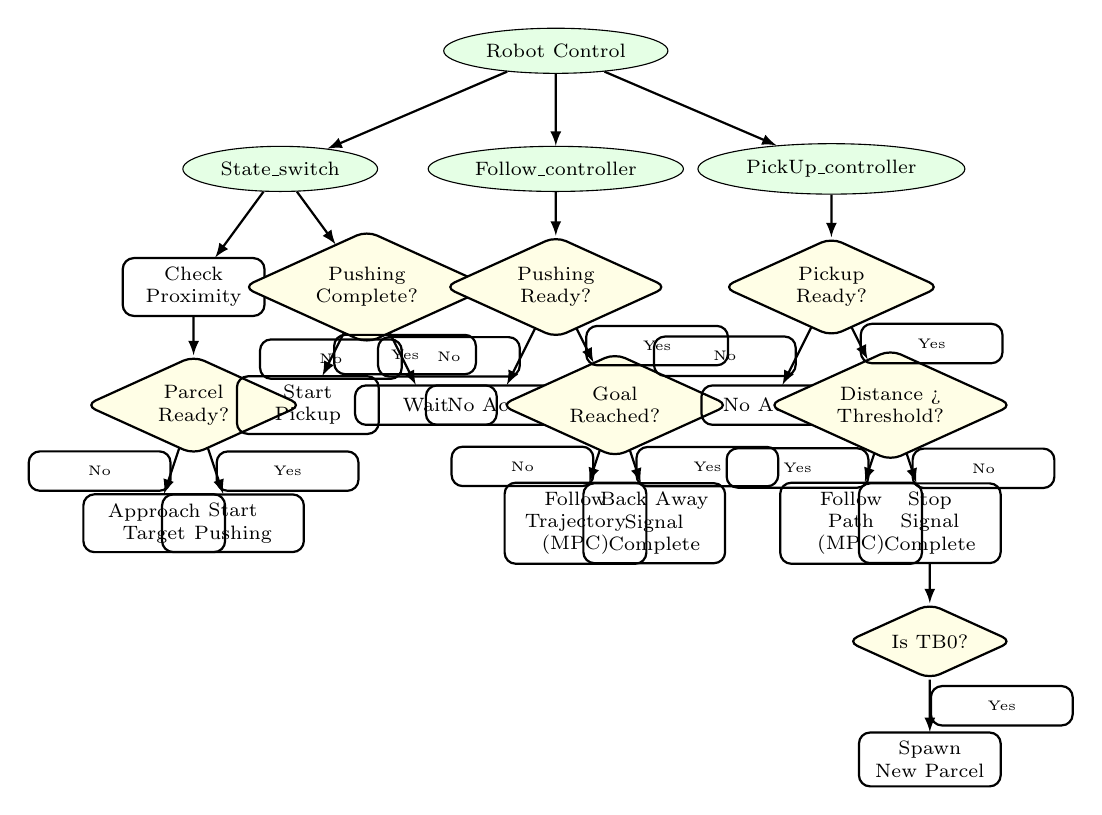
\begin{tikzpicture}[
  level 1/.style={sibling distance=35mm},
  level 2/.style={sibling distance=22mm},
  level 3/.style={sibling distance=15mm},
  level 4/.style={sibling distance=10mm},
  every node/.style={draw, rounded corners, minimum height=5mm, minimum width=18mm, align=center, font=\scriptsize},
  edge from parent/.style={draw, -latex, thick},
  decision/.style={draw, diamond, aspect=2.2, fill=yellow!10, align=center, font=\scriptsize},
  state/.style={draw, ellipse, fill=green!10, align=center, font=\scriptsize}
]

% Root node and first level
\node[state] {Robot Control}
  child {
    node[state] {State\_switch}
    child {
      node {Check\\Proximity}
      child {
        node[decision] {Parcel\\Ready?}
        child {
          node {Approach\\Target}
          edge from parent node[left, font=\tiny] {No}
        }
        child {
          node {Start\\Pushing}
          edge from parent node[right, font=\tiny] {Yes}
        }
        edge from parent
      }
      edge from parent
    }
    child {
      node[decision] {Pushing\\Complete?}
      child {
        node {Start\\Pickup}
        edge from parent node[right, font=\tiny] {Yes}
      }
      child {
        node {Wait}
        edge from parent node[left, font=\tiny] {No}
      }
      edge from parent
    }
    edge from parent
  }
  child {
    node[state] {Follow\_controller}
    child {
      node[decision] {Pushing\\Ready?}
      child {
        node {No Action}
        edge from parent node[left, font=\tiny] {No}
      }
      child {
        node[decision] {Goal\\Reached?}
        child {
          node {Follow\\Trajectory\\(MPC)}
          edge from parent node[left, font=\tiny] {No}
        }
        child {
          node {Back Away\\Signal\\Complete}
          edge from parent node[right, font=\tiny] {Yes}
        }
        edge from parent node[right, font=\tiny] {Yes}
      }
      edge from parent
    }
    edge from parent
  }
  child {
    node[state] {PickUp\_controller}
    child {
      node[decision] {Pickup\\Ready?}
      child {
        node {No Action}
        edge from parent node[left, font=\tiny] {No}
      }
      child {
        node[decision] {Distance >\\Threshold?}
        child {
          node {Follow\\Path\\(MPC)}
          edge from parent node[left, font=\tiny] {Yes}
        }
        child {
          node {Stop\\Signal\\Complete}
          child {
            node[decision] {Is TB0?}
            child {
              node {Spawn\\New Parcel}
              edge from parent node[right, font=\tiny] {Yes}
            }
            edge from parent
          }
          edge from parent node[right, font=\tiny] {No}
        }
        edge from parent node[right, font=\tiny] {Yes}
      }
      edge from parent
    }
    edge from parent
  };
\end{tikzpicture}
}
\caption{Robot Control Action Tree}
\end{figure}

\begin{figure}[h]
\centering
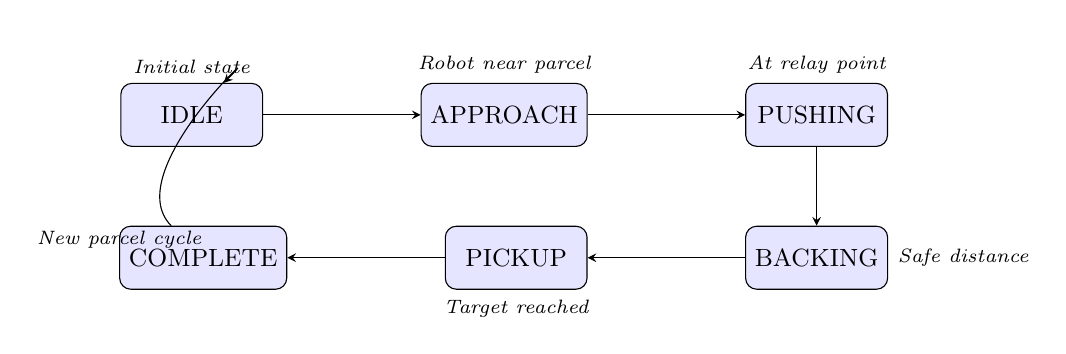
\begin{tikzpicture}[
  node distance=1cm,
  state/.style={rectangle, rounded corners, draw=black, minimum height=8mm, minimum width=18mm, fill=blue!10, font=\small},
  arrow/.style={->, >=stealth},
  note/.style={font=\scriptsize\itshape}
]

% States
\node[state] (idle) {IDLE};
\node[state, right=2cm of idle] (approach) {APPROACH};
\node[state, right=2cm of approach] (pushing) {PUSHING};
\node[state, below=1cm of pushing] (backing) {BACKING};
\node[state, left=2cm of backing] (pickup) {PICKUP};
\node[state, left=2cm of pickup] (complete) {COMPLETE};

% Connect the states
\draw[arrow] (idle) -- (approach);
\draw[arrow] (approach) -- (pushing);
\draw[arrow] (pushing) -- (backing);
\draw[arrow] (backing) -- (pickup);
\draw[arrow] (pickup) -- (complete);
\draw[arrow] (complete) to[out=135,in=45,looseness=1.3] (idle);

% Add notes
\node[note, above=0mm of idle] {Initial state};
\node[note, above=0mm of approach] {Robot near parcel};
\node[note, above=0mm of pushing] {At relay point};
\node[note, right=0mm of backing] {Safe distance};
\node[note, below=0mm of pickup] {Target reached};
\node[note, above=0mm of complete.west] {New parcel cycle};

\end{tikzpicture}
\caption{Robot Control State Machine}
\end{figure}

\begin{figure}[h]
\centering
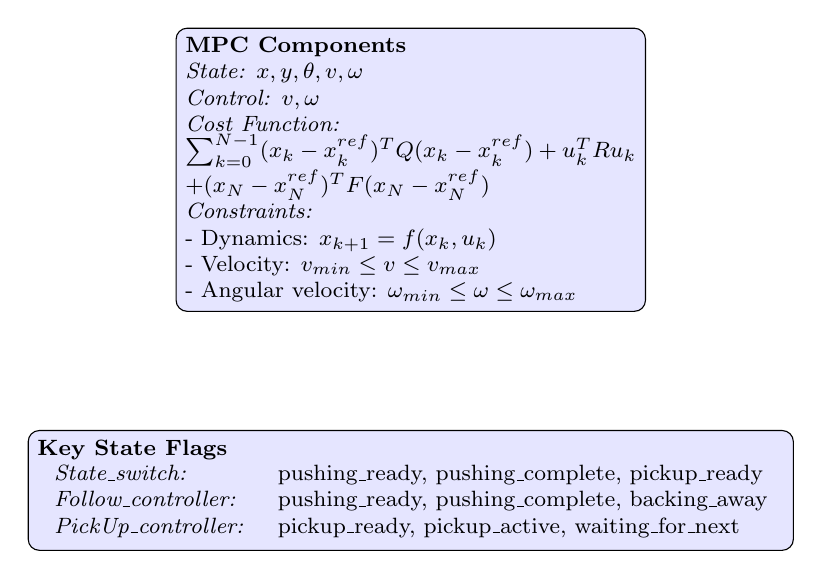
\begin{tikzpicture}[
  node distance=1cm,
  box/.style={rectangle, draw, rounded corners, fill=blue!10, align=center, font=\footnotesize},
  arrow/.style={->, >=stealth}
]

\node[box, align=left] (mpc) {
\textbf{MPC Components}\\
\textit{State:} $x, y, \theta, v, \omega$\\
\textit{Control:} $v, \omega$\\
\textit{Cost Function:}\\
$\sum_{k=0}^{N-1}(x_k-x_k^{ref})^TQ(x_k-x_k^{ref}) + u_k^TRu_k$\\
$+(x_N-x_N^{ref})^TF(x_N-x_N^{ref})$\\
\textit{Constraints:}\\
- Dynamics: $x_{k+1} = f(x_k,u_k)$\\
- Velocity: $v_{min} \leq v \leq v_{max}$\\
- Angular velocity: $\omega_{min} \leq \omega \leq \omega_{max}$
};

\node[box, below=1.5cm of mpc, align=left] (pseudo) {
\textbf{Key State Flags}\\
\begin{tabular}{ll}
\textit{State\_switch:} & pushing\_ready, pushing\_complete, pickup\_ready\\
\textit{Follow\_controller:} & pushing\_ready, pushing\_complete, backing\_away\\
\textit{PickUp\_controller:} & pickup\_ready, pickup\_active, waiting\_for\_next
\end{tabular}
};

\end{tikzpicture}
\caption{MPC Formulation and State Management}
\end{figure}

\end{document}
